\documentclass[11pt]{article}
\usepackage[utf8]{inputenc}
\usepackage{relsize}
\usepackage[margin=1in]{geometry}
\usepackage{graphicx}
\usepackage{wrapfig}
\usepackage[none]{hyphenat}
\usepackage{enumitem}
\usepackage{hyperref}
\hypersetup{
    colorlinks=true,% make the links colored
}


\usepackage{xcolor} % to access the named colour LightGray
\definecolor{LightGray}{gray}{0.9}

\usepackage{amsmath}
\usepackage[utf8]{inputenc}
\usepackage[english]{babel}
\usepackage{caption}

\usepackage[newfloat]{minted}
\captionsetup[listing]{position=top}
\DeclareMathOperator{\arctg}{arctg}

\usepackage{hyperref}
\hypersetup{
    colorlinks=true,
    linkcolor=blue,
    filecolor=magenta,      
    urlcolor=blue,
    pdftitle={Overleaf Example},
    pdfpagemode=FullScreen,
    }

\urlstyle{same}



\begin{document}

\begin{titlepage}
    \begin{center}
        
\includegraphics[scale=1]{DU-log.png} \\[12pt]
        
        \Huge \textbf{University of Dhaka}
        \begin{center}
           { \LARGE \textbf{Department of Computer Science and Engineering \\[8pt]}}
           
             {\textbf{ \huge CSE-3113:\\[8pt]}}

             
             {\textbf{ \huge Microprocessor and Assembly Language Lab	 \\[8pt]}}
             
                        
             \begin{huge}
                    \textbf{ \huge Lab Report 5\\[8pt]}
                 
        		\textbf{Submitted By:\\[8pt]}
        			 Syed Mumtahin Mahmud, Roll: 50\\[8pt]
        		\textbf{Submitted On : \\[8pt]}
        			March 8, 2023\\[10pt]
        		\textbf{Submitted To :\\[8pt]}
        			Dr. Upama Kabir \\[8pt]
                        Dr. Md. Mustafizur Rahman\\[8pt]
                      
	       \end{huge}
             
        \end{center}
    \end{center}
\end{titlepage}
\begin{Large}
\title{\huge Table of Contents}

\maketitle
\hypersetup{linkcolor=black}
\tableofcontents
\end{Large}

\newpage
\section{Objectives}
The objectives of this lab is to understand and have familiarize with register based assembly programming for Cortex M4 processor for handling non-recursive, recursive and nested function call.  \\[10pt]

When a function is called, the control of the program is transferred from the caller to the callee. The callee performs the required task and returns the control to the caller.  \\[10pt]

In the ARM Cortex M4 architecture, the BL (branch and link) instruction is used to call a function. The LR (link register) is used to store the return address. At the end of the function call, the MOV (move) instruction is used to move the value of LR into the PC (program counter) register to return the control to the caller.  \\[10pt]

However, to handle the function call correctly, the ARM Procedure Call Standard (APCS) must be followed. In the APCS, registers R0-R3 are used to pass argument values into a function and to return a result value from a function. They can also be used to hold intermediate values within a function.  \\[10pt]

Register R12 (IP) may be used by a linker as a scratch register between a main function and any other functions it calls. It can also be used within a routine to hold intermediate values between function calls. Registers R4-R8, R10, and R11 are used to hold the values of a function's local variables. However, if a called function needs these registers for extra workspace, it must preserve their contents by saving them on the stack. \\[10pt]

In the ARM Cortex M4 architecture, registers R12-R15 have special roles and are labeled IP, SP, LR, and PC. The memory of a process can be classified into five categories: code, read-only static data, writable static data, the heap, and the stack. The stack is used to save the contents of registers when they need to be preserved during function calls, as registers are limited in number compared to memory.  \\[10pt]
\section{Lab Tasks}
\subsection{Question 1}
Write an assembly language program to identify prime numbers from a list of array by calling a function called prime.
\begin{listing}[h]
    \caption{Adding 3 NumbersLogical operations on two 16-bit variables}
    \begin{minted}[linenos,frame=single]{nasm}
         AREA arr_dec, DATA, READWRITE

numbers DCD 7,4,3,5
prm DCD 0,0,0,0
	
	AREA prime_number,CODE,READONLY
	ENTRY
	EXPORT main
prime
	PUSH {R3,R4,R5,R6}
	MOV R4,#2 ;divisor start from 2
	CMP R0,#2
	BLT not_prime
is_prime
	CMP R0,R4 ;check if the R4 is reached the value of R0
	BEQ prime_cnf
	SDIV R5,R0,R4
	MUL R5,R5,R4 
	CMP R0,R5
	BEQ not_prime
	ADDS R4,R4,#1 ; increase R4
	B is_prime
prime_cnf
	POP {R3,R4,R5,R6}
	STR R0,[R3],#4
	BX LR
	ENDP

not_prime
	POP {R3,R4,R5,R6}
	BX LR
	ENDP
main
	LDR R3,=prm
	LDR R4,=numbers
	MOV R5,#4 ;size of array
	MOV R6,#4 ;size of array
loop
	LDR R0,[R4],#4
	BL prime
	SUB R6,R6,#1
	CMP R6,#0
	BNE loop
	
stop B stop ; end of code
	END

\end{minted}
\end{listing}


\clearpage
\begin{figure}[!h]
    \centering
    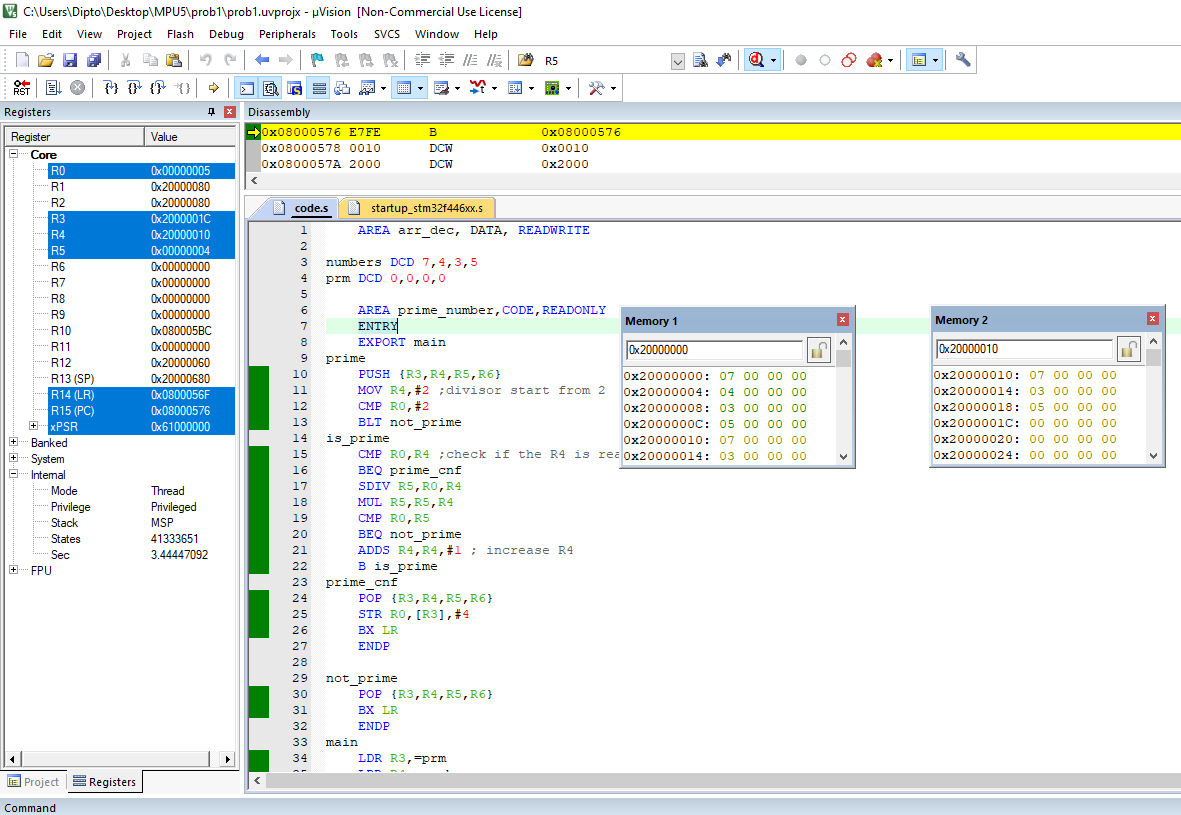
\includegraphics[width=\textwidth]{prob1.PNG}
    \caption{program to identify prime numbers from a list of array}
\end{figure} 
\clearpage


\subsection{Question 2}
Write an assembly language program to perform the summation of two numbers by call a function sum(arg1, arg2) using call-by-value\\
\begin{listing}[h]
    \caption{Summation of two numbers by call a function using call-by-value}
    \begin{minted}[linenos,frame=single]{nasm}
    AREA p_two, CODE, READONLY
    ENTRY
    EXPORT main
        
sum_function PROC ;sum function 
    ; Retrieve arguments from the stack
    POP {r3,r4} ; arg1 arg2

    ; Add the arguments
    ADD r0, r3, r4
    PUSH {r0}

    ; Return the result
    BX lr
	ENDP

main
    ; Initialize arguments
    MOV r1, #3 ; arg1 = 3
    MOV r2, #2 ; arg2 = 2
    
    PUSH {lr} ; Save the return address
    PUSH {r1, r2} ; Push arguments onto the stack
    BL sum_function ; Call the function
    POP {r5} ; Pop result arguments from the stack

    POP {pc} ; Pop the return address into pc
     
    B Stop
Stop B Stop ; Infinite loop to halt the program
	END
\end{minted}
\end{listing}

\clearpage
\begin{figure}[!h]
    \centering
    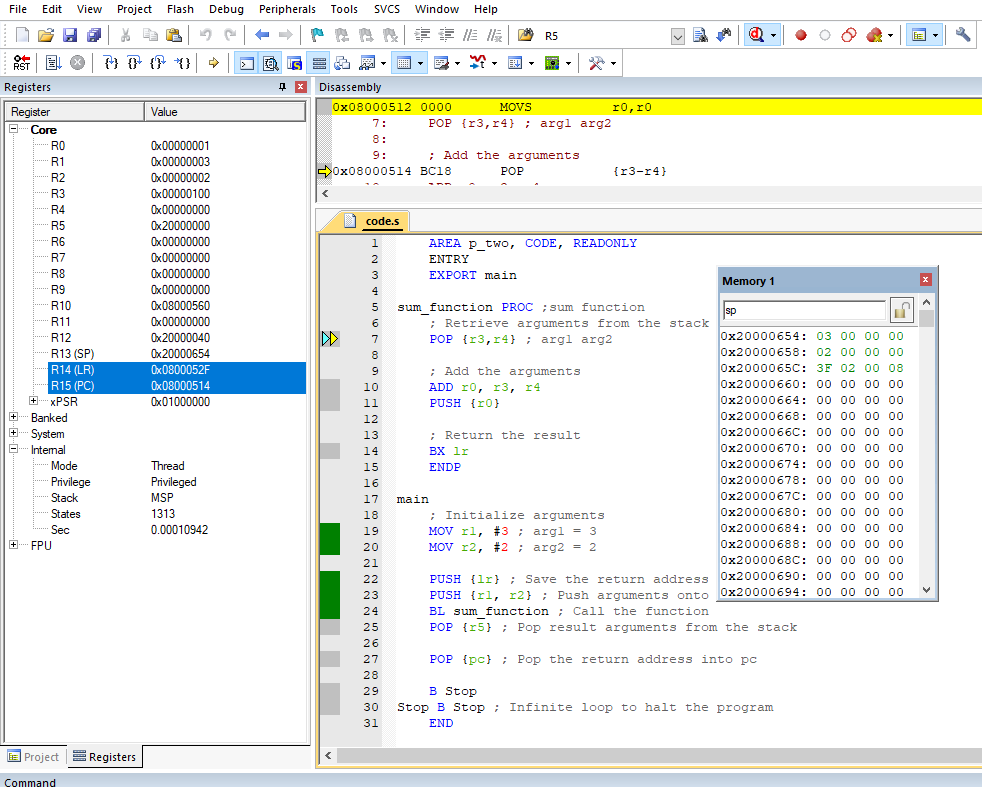
\includegraphics[width=\textwidth]{prob2.PNG}
    \caption{summation of two numbers}
\end{figure} 
\clearpage


\subsection{Question 3}
Write an assembly language program to perform the summation of two numbers by call a function sum(arg1, arg2) using call-by-reference.
\begin{listing}[h]
    \caption{summation of two numbers by call a function using call-by-reference.}
    \begin{minted}[linenos,frame=single]{nasm}
	AREA dec, DATA, READWRITE
num1 DCD 2 ;first number
num2 DCD 3 ;second number
result DCD 0 ;result variable
	AREA main_prog, CODE, READONLY
	ENTRY
	EXPORT main
		
sum
	POP {R3,R4,R5}
    LDR R3, [R3] ;load arg1 from memory
    LDR R4, [R4] ;load arg2 from memory
    ADD R3, R3, R4 ;add arg1 and arg2
    STR R3, [R5] ;store the result in memory
	BX lr
    ENDP
	
main
	LDR R0, =num1 ;address of first number
	LDR R1, =num2 ;address of second number
	LDR R2, =result ;address of result variable
	PUSH {R0,R1,R2}
	BL sum ;call the sum function
	LDR R2,[r2]
	B stop ;end of program
	

	
stop B stop ;end of code
	END

\end{minted}
\end{listing}
\clearpage
\begin{figure}[!h]
    \centering
    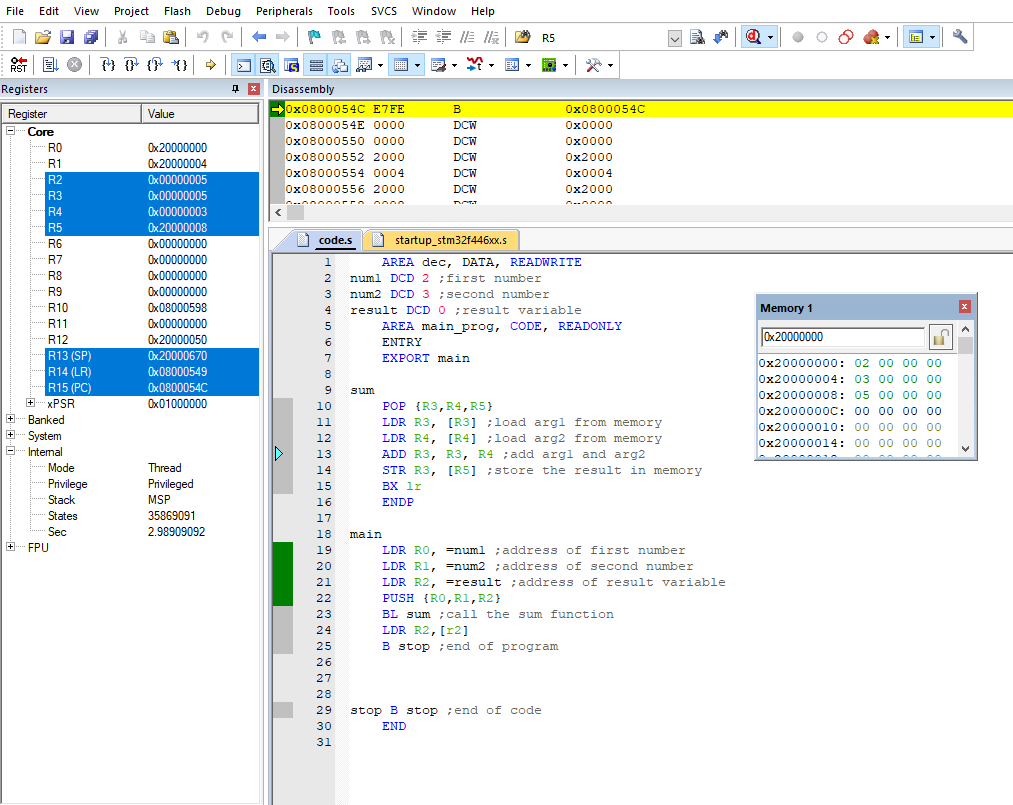
\includegraphics[width=\textwidth]{prob3.PNG}
    \caption{summation of two numbers}
\end{figure} 
\clearpage
\subsection{Question 4}
Write an assembly language program to find and return the minimum element in an array, where the array and its size are given as parameters by using recursive function.
\begin{listing}[h]
    \caption {program to find and return the minimum element in an array}
    \begin{minted}[linenos,frame=single]{nasm}
		AREA arr_min, DATA, READWRITE
arr DCD 10, 5, 8, 3, 6, 2, 7 ;example array
arr_size EQU 7 ;size of example array
	
	AREA min_elem, CODE, READONLY
	ENTRY
	EXPORT main
	EXPORT find_min
find_min
	POP{R3,R1}
	CMP R1,#0
	BEQ ret
	LDR R2,[R0],#4
	CMP R2, R3        ; compare current element with minimum value
    MOVLT R3, R2      ; if current element is smaller, update minimum value
	SUBS R1,R1,#1
	PUSH {R3,R1}
	BL find_min
ret   
	POP {pc}
main
    LDR R0, =arr ;load the address of the array
    LDR R1, =arr_size ;load the size of the array
	MOV r3,#100 ;initializing min element
	PUSH{lr,r3,r1}
    BL find_min ;call the function to find the minimum element
    MOV R1, R0 ;move the result to R1
    B stop ;end of program
stop B stop ;end of code
	END
\end{minted}
\end{listing}
\clearpage
\begin{figure}[!h]
    \centering
    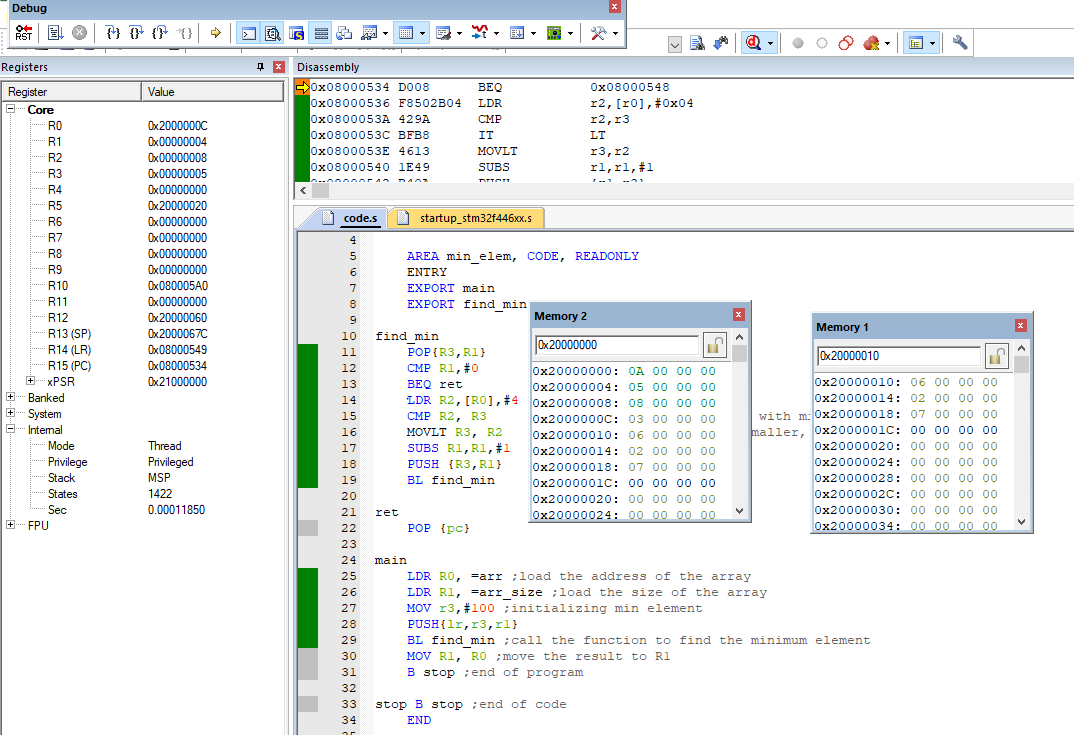
\includegraphics[width=\textwidth]{prob4.PNG}
    \caption{find and return the minimum element in an array}
\end{figure} 
\clearpage
\subsection{Question 5}
Write an assembly language program to perform the nested function call.
\begin{listing}[h]
    \caption{ Find the largest among n different numbers}
    \begin{minted}[linenos,frame=single,escapeinside=~~]{nasm}
    AREA p_two, CODE, READONLY
    ENTRY
    EXPORT main
sum_function  
    ; Retrieve arguments from the stack
    POP {r3,r4} ; arg1 arg2
	push{lr}
    ; Add the arguments
    ADD r0, r3, r4
    PUSH {r0}
    BL sub_func
	ENDP	
sub_func
	POP {r1}
	pop{lr}
	SUB r1,r1,#1
	push{r1}
	BX lr
main
    ; Initialize arguments
    MOV r1, #3 ; arg1 = 3
    MOV r2, #2 ; arg2 = 2
    PUSH {r1, r2} 
    BL sum_function 
    POP {r5} 
    B Stop
Stop B Stop 
	END

        .
\end{minted}
\end{listing}

\clearpage
\begin{figure}[!h]
    \centering
    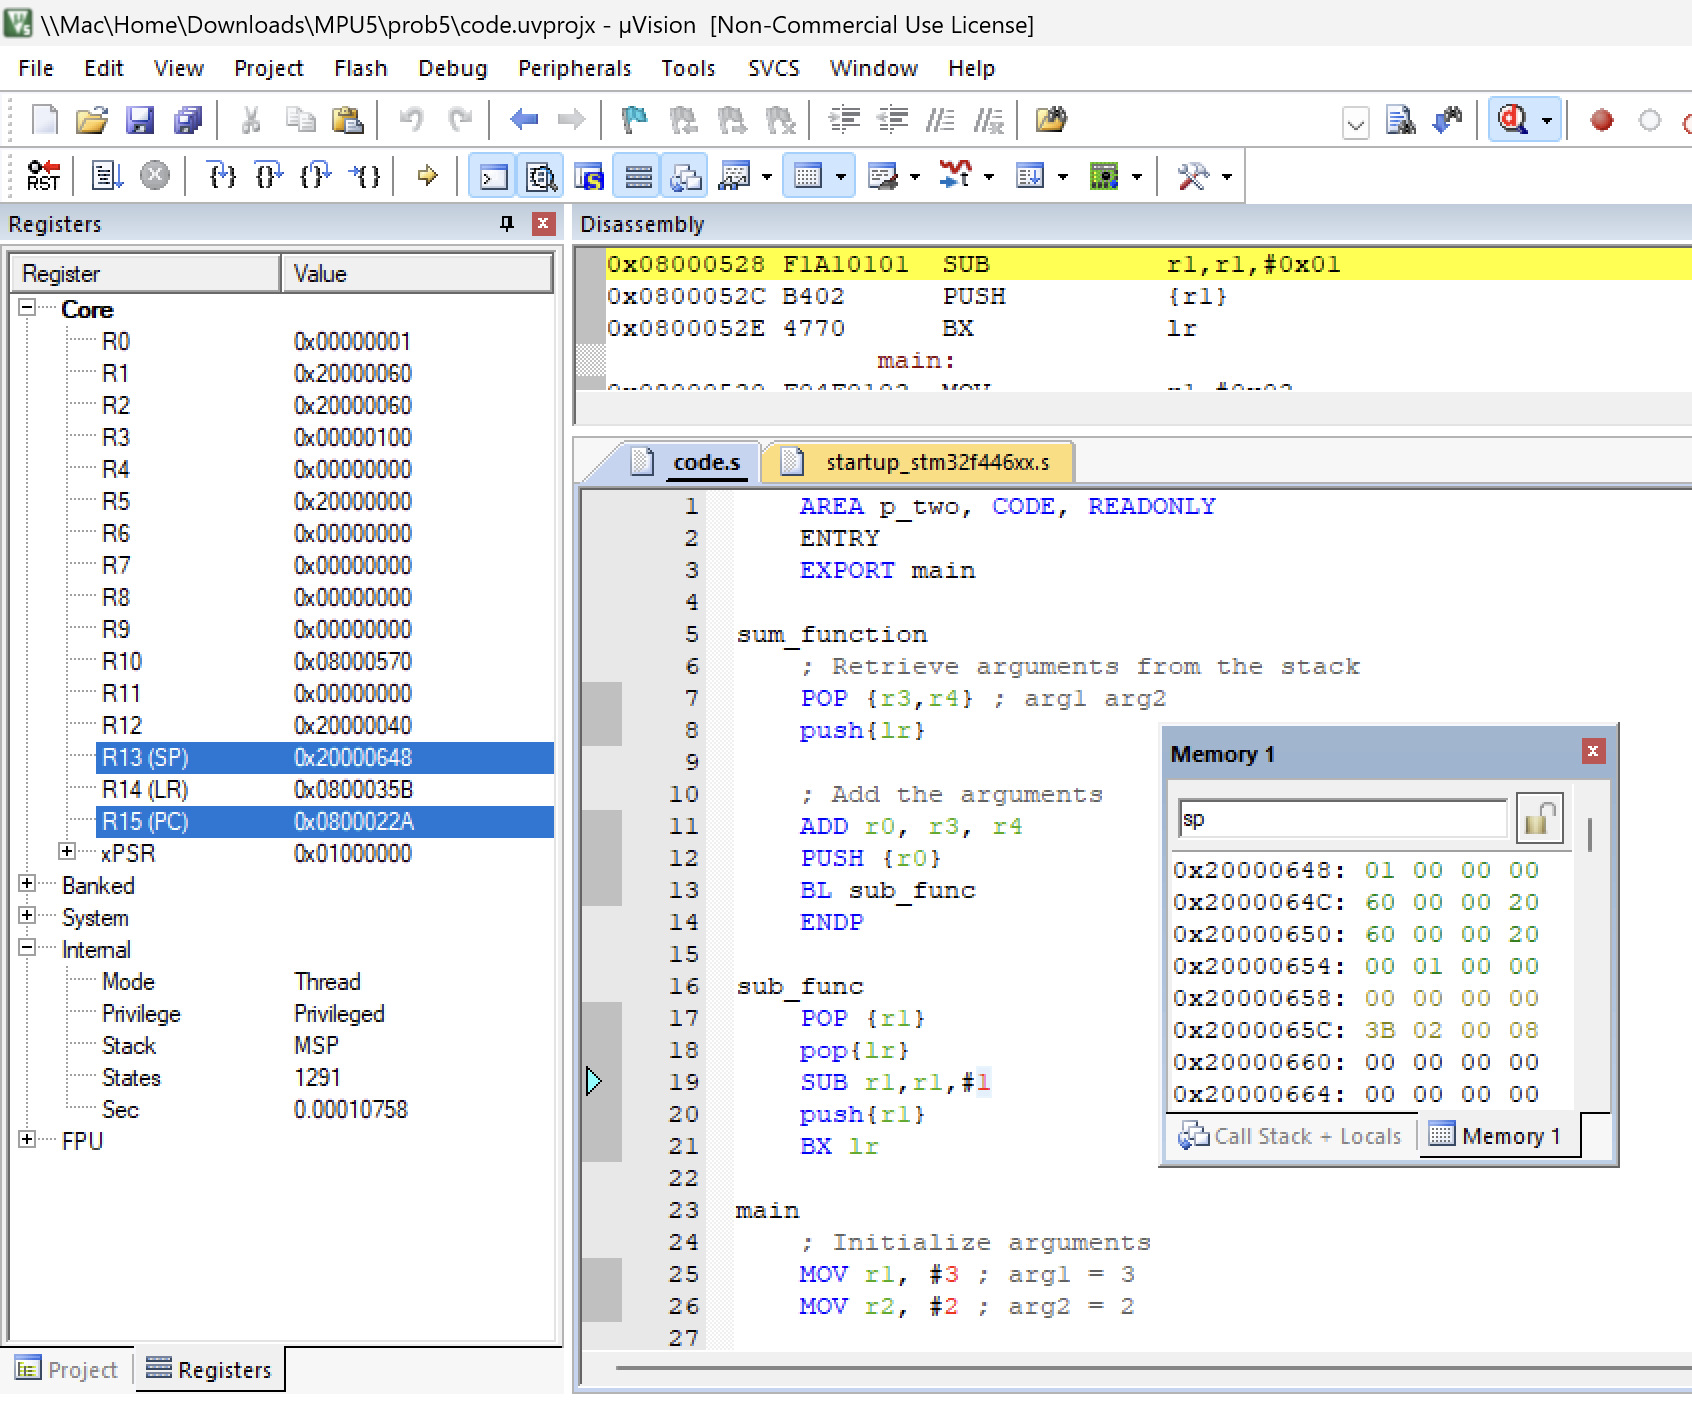
\includegraphics[width=\textwidth]{prob5.png}
    \caption{Program to perform the nested function call.}
\end{figure} 

\newpage
\bibliographystyle{plain}
\bibliography{refs}
\nocite{*}


\end{document}